Рассмотрим задачу определения новых положений узлов расчетной сетки, если для каждого узла $\vec{N}$ известна скорость нарастания льда $v(\vec{N})$ в метрах в секунду.
Будем считать, что нарастание льда в любой точке роста выполняется одновременно во всех направлениях аналогично принципу Гюйгенса-Фреленя распространения волн.
Тогда фронт распространения льда от произвольной точки $\vec{P}$ через промежуток времени $\Delta t$ будет иметь форму сферы с центром в точке $\vec{P}$ и радиусом $v(\vec{P}) \Delta t$.
Далее будем предполагать, что выполняется расчет новых положений узлов через некоторый фиксированный момент времени $\Delta t$, то есть для каждого узла известен радиус продвижения фронта льда $R(\vec{N}) = v(\vec{N}) \Delta t$.
Так как элементами расчетной сетки являются треугольники, но необходимо определить радиус продвижения фронта льда для каждой внутренней точки треугольника по данным его вершин.

Рассмотрим ячейку расчетной сетки, вершинами которой являются точки $\vec{A}$, $\vec{B}$, $\vec{C}$ (каждая точка представлена вектором в трехмерном пространстве).
Точки треугольника представляют собой геометрическое место точек, описываемое следующим образом:

\begin{equation}
\begin{cases}
\vec{P}(\beta, \gamma) = \vec{A} + \beta (\vec{B} - \vec{A}) + \gamma (\vec{C} - \vec{A}) = \vec{A} + \beta \vec{AB} + \gamma \vec{AC} \\
\beta \ge 0 \\
\gamma \ge 0 \\
\beta + \gamma \le 1
\end{cases}
\end{equation}

Определим для каждой точки треугольника $\vec{P}(\beta, \gamma)$ радиус продвижения фронта льда как $R(\vec{P}(\beta, \gamma)) = R(\beta, \gamma) = R(\vec{A}) + \beta (R(\vec{B}) - R(\vec{A})) + \gamma (R(\vec{C}) - R(\vec{A})) = R_A + \beta R_{AB} + \gamma R_{AC}$.
Фронт продвижения льда от точки $\vec{P}(\beta, \gamma)$ представляет собой сферу $S(\beta, \gamma) = S(\vec{P}(\beta, \gamma), R(\beta, \gamma))$.
Фронтом продвижения льда всей треугольной ячейки будем считать общую огибающую сфер, построенных на всех точках этой ячейки.

\begin{figure}[h]
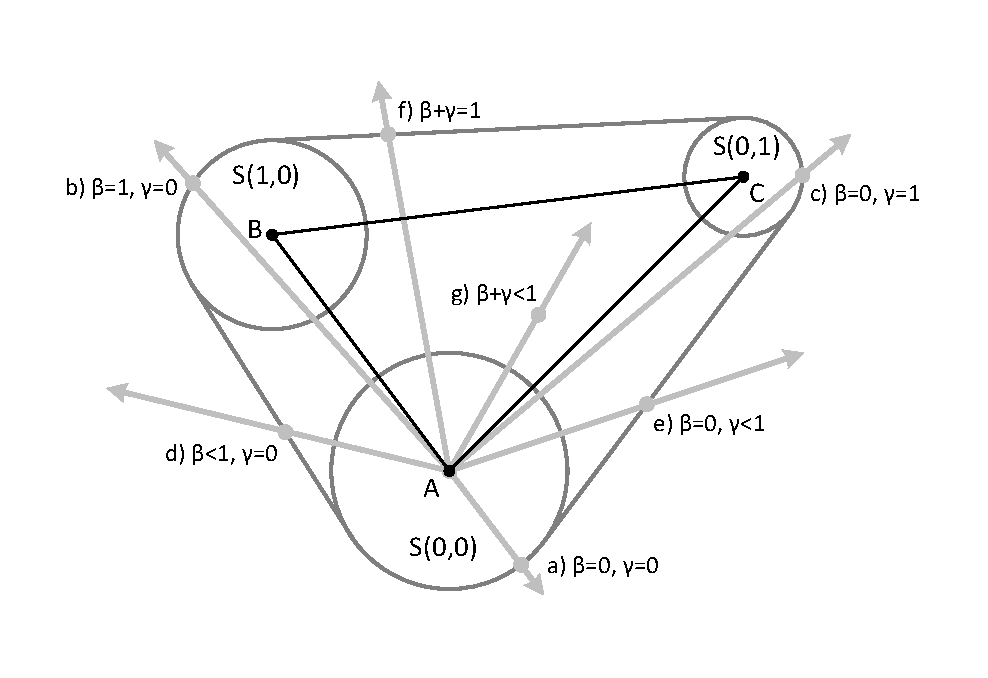
\includegraphics[width=0.6\textwidth]{pics/pic_general_envelope_size.pdf}
\captionstyle{center}\caption{Общая огибающая TODO.}\label{fig:pic_gereral_envelope_size}
\end{figure}
